%\section{Hetergeneous Access Point Band Selection}
%\label{sec:moa_problemformulation}
%
%% Introduce the content of this section
%In this section, we illustrate the challenges of hetergenous access point 
%band selection in wireless network deployment and formulate the problem of band 
%selection in mesh network deployments jointly using WiFi and white space bands. 
%Further, we present a linear program and MHAPD(Multiband Hetergeneous AP Deployment) algorithm for estimating the 
%access point number to serve the traffic demand of a given population.
%Then we discuss the application of the algorithm in uniform population
%distribution and non-uniform population distribution with spectrum resource 
%variation to tell the general rules in picking up channels for access points.
 
%\subsection{White Space Opportunity and Challenge}
%\label{subsec:motivation}

%% Propagation
%Wireless propagation is the behavior of the signal loss characteristics 
%when wireless signals are transmitted through the wireless medium.
%The strength of the received signal depends on both the line-of-sight
%path (or lack thereof) and multiple other paths that result from 
%reflection, diffraction, and scattering from 
%obstacles~\cite{andersen1995propagation}. The widely-used Friis
%equation characterizes the received signal power $P_r$ in terms 
%of transmit power $P_t$, transmitter gain $G_t$, receiver gain $G_r$, 
%wavelength $\lambda$ of the carrier frequency, 
%distance $R$ from transmitter to receiver, and path loss exponent 
%$n$ according to~\cite{friis}:
%\begin{equation}
%\label{eq:friis}
%P_r=P_t+G_t+G_r+10n \log_{10}\left( \frac{\lambda}{4\pi R}\right)
%\end{equation}
%Here, $n$ varies according to the aforementioned environmental 
%factors with the value of two to five in typical outdoor 
%settings~\cite{rappaport}.

% Hetergenous access points
%Despite sufficient levels of received signal, interference can cause channels
%to be unusable (e.g., due to high levels of packet loss) or unavailable (e.g.,
%due to primary users in cognitive radios~\cite{haykin2005cognitive}).
%Prior work has worked to reduce cost through gateway deployment, channel 
%assignment, and routing~\cite{he2008optimizing,tang2005interference}.
%Most of existing works try to reduce the intra-network interference or increase
%the channel usability level of wireless network deployment
%~\cite{si2010overview,joshi2009efficient}. However, the access point service area
%variation becomes an important problem when considering the availability of white space bands.  
%Jointly considering the propagation and single channel capacity, the access points 
%with different configuration (e.g. radios) in the same area, or with same configuration 
%in diverse population density areas (e.g. downtown, rural) could have different service ranges.
%
%% Explain multiband and hetergenous access points
%When wireless devices operate in WiFi bands, the channel separation is relatively
%small (e.g., 22 MHz for the 2.4 GHz band). As a result, many works assume that
%the propagation characteristics across channels are similar. However, with the
%large frequency gaps of WiFi and white space bands (e.g., several GHz),
%propagation becomes a key factor in the deployment of wireless networks with both bands.
%Here, a frequency band is defined as a group of channels which have
%small separation meaning similar propagation characteristics.
%In this work, we consider the diverse propagation and activity characteristics
%for four total frequency bands: 450 MHz, 800 MHz, 2.4 GHz, and 5.2 GHz.
%We refer to the two former frequency bands as white space bands and
%the two latter frequency bands as WiFi bands.
%A general way to increase the capacity of a single access point is to add channels
%through radios~\cite{raniwala2005architecture}. The assumption all the channels have
%the same propagation does not fit for WiFi and white space hetergenous scenario.
%When a white space band channel added to an access point, the capacity and service 
%range could increase simultaneously. The differences in propagation and constraints 
%of network deployment create opportunity for the joint use of white space and 
%WiFi bands in wireless access networks according to the environmental characteristics 
%(e.g., urban or rural and downtown or residential) of the deployment location.
%
%% Network Constraints
%Typically, the deployment of wireless access networks is subject to coverage and capacity
%constraints for a given region. Coverage is defined with respect to the ability of
%clients to connect to access points within their service area.  We use a coverage
%constraint ratio of $95\%$ in this work for a target area~\cite{robinson2010deploying}.
%Capacity is defined with respect to the ability of a network to serve the traffic 
%demand of clients.  Spatial reuse allows improved capacity, but increases the cost
%of deploying a network by increasing the total number of access points required.
%Hence, for densely populated areas the greatest level of spatial reuse possible
%is often desired. And the deployment cost could be significant reduced through access 
%points with high capacity with more centralized using radios. In contrast, 
%sparsely-populated rural areas have lower traffic demand per unit area. Thus, 
%aggregating this demand with lower-frequency, white space bands could be highly 
%effective in reducing the total number of access points required to achieve 
%similar coverage and capacity constraints. Moreover, since less TV channels tend
% to be occupied in sparsely populated areas~\cite{msdatabase}, a larger number 
% of white space bands can be leveraged in these areas. 

% More variation in population distribution



\section{Hetergeneous Access Point Band Selection}
\label{subsec:moaproblem}

% Assumptions of the network
As opposed to previous works such as
~\cite{franklin2007node,robinson2010deploying,si2010overview}, 
this paper focuses on hetergenous access point selection 
for wireless access networks which jointly employ WiFi and white space bands.
We propose a relaxed linear program to find the lower bound number of access point,
and MHAPD algorithm  to approach the lower bound number of access points which serve
the traffic demand of a certain area. We assume the service provider has a limited number 
of spectrum resources and radios have similar configuration. Each radio on an access 
point operates with a classic protocol model~\cite{gupta2000capacity}. 
We further assume that there is a given take rate and traffic demand for a given 
population (as specified in Section~\ref{sec:moaexperimentdesign}).

%% Capacity constraint
%A network deployment should ideally provide network capacity equal to the demand of the service 
%area to maintain the capacity constraint. The demand of a service area could be calculated as the 
%summation of individual demands all over the service area $D_a=\sum_{p\in P}D_p$. Since 
%household demand for Internet has been previously characterized~\cite{rosston2011household}, 
%$D_a$ could represent the population distribution $f$ and service area $k$ as 
%$D_a=\sum_{f \in F,k \in K}\bar{D_p}*f*k$. 
%The capacity constraint could be represented with access points set $M$ according to:
%\begin{equation}
%\label{eq:nlbound}
%\sum_{m \in M}C_r^m \ge \sum_{f \in F,k \in K}\bar{D_p}*f*k
%\end{equation}
%% Coverage constraint
%At the same time, the wireless network must additionally satisfy the coverage constraint in the service 
%area where the access points provide connectivity for client devices. 
%Generally, a coverage of $95\%$ is acceptable for wireless access networks~\cite{robinson2010deploying}.
%The object of this work is to find the best possible number of access points so that the network has good 
%connectivity and enough capacity to satisfy the traffic demands.


% Hetergeneous Access point & resource constraint
Under the capacity and coverage constraints, the serveice area of a hetergeneous multiband access point 
varies according to the traffic demand. The service area is limited by the propagation range when the traffic 
demand is low; and when the traffic demand is high, the service area is limited by the radio capacity.
The radius of service area $r_s$ could be represented as:
\begin{equation}
\label{eq:servicearea}
r_s=min\{r_p,r_c\}
\end{equation}
$r_p$ represents the propagation range of a radio in the access point, $r_c$ is the capacity range of 
a a radio in the access point. When the traffic demand is distributed uniform in a circle, from 
Eq.~\ref{eq:nlbound} the capacity range $r_c$ could be noted as $r_c=\sqrt{k/\pi}$. Moreover,
the propagation range and capacity rang could be determined by the environment, traffic distribution and
power control~\cite{robinson2010deploying}. These factors are out of the scope of this work, but they could
easily be added to the model for calculation of a hetergenous access point service area. To simplify the 
problem and focus on multiband, we assume the traffic demand is uniform distributed and the propagation 
follow Frii rule as Eq.~\ref{eq:friis}. When the target area is given, we could get the service area of
each access point type through~\ref{eq:servicearea}, then we adjust the transmit power of each radio
to reduce the interference among each other.

% Variation of radios
When the traffic demand of an area is constant, the degree of a hetergenous access point service area 
varies with the radios. We assume all the access points have the same number of radios and channel 
resources.
% Lower traffic demand case
In the low traffic demand scenario, the service radius reaches the radio propagation range.
A high frequency WiFi radios will have a smaller service area since the signal attenuate fast; while the white
space radio could have a larger service area due to the longer propagation; and a hetergenous access point who has
both WiFi radios and white space radios has the same range of as low frequency radios access point. An example is
shown in Fig.~\ref{fig:lowtraffic}.
% Medium traffic demand case
In medium traffic demand scenario, hetergenous access points and white space access points will 
have the same size service area which is larger than high frequency WiFi only access points as shown in 
~\ref{fig:mediumtraffic}.
% High traffic demand case
With high traffic demand, all access points will have the same service area due to capacity constraint 
as shown in~\ref{fig:hightraffic}. White space bands could reduce the cost of wireless network deployment. 
Thus, lowest cost for covering a certain area is to use white space bands in all access points 
based on the analysis. However, spectrum resource is limited, especially the usability
of white space bands is restricted in major cities in US~\cite{msdatabase}. 
% Problem
Thus, the trade of between centralized using all white space bands or mixed using white space
bands under multiple traffic demands is a question for wireless network deployment. The problem
could be modeled as how could we use the minumum number of different sizes of service area according to 
radio combinations to cover a certain plane area. This problem is a to deploy different size of cells in 
a given palen, which is a NP-hard bin package problem~\cite{martello1998exact}. We propose a relaxed 
linear program to get the lower bound of the number of access points and a heuristic algorithm to 
approach the lower bound.



\begin{figure}[h]
%\vspace{-0.0in}
\centering
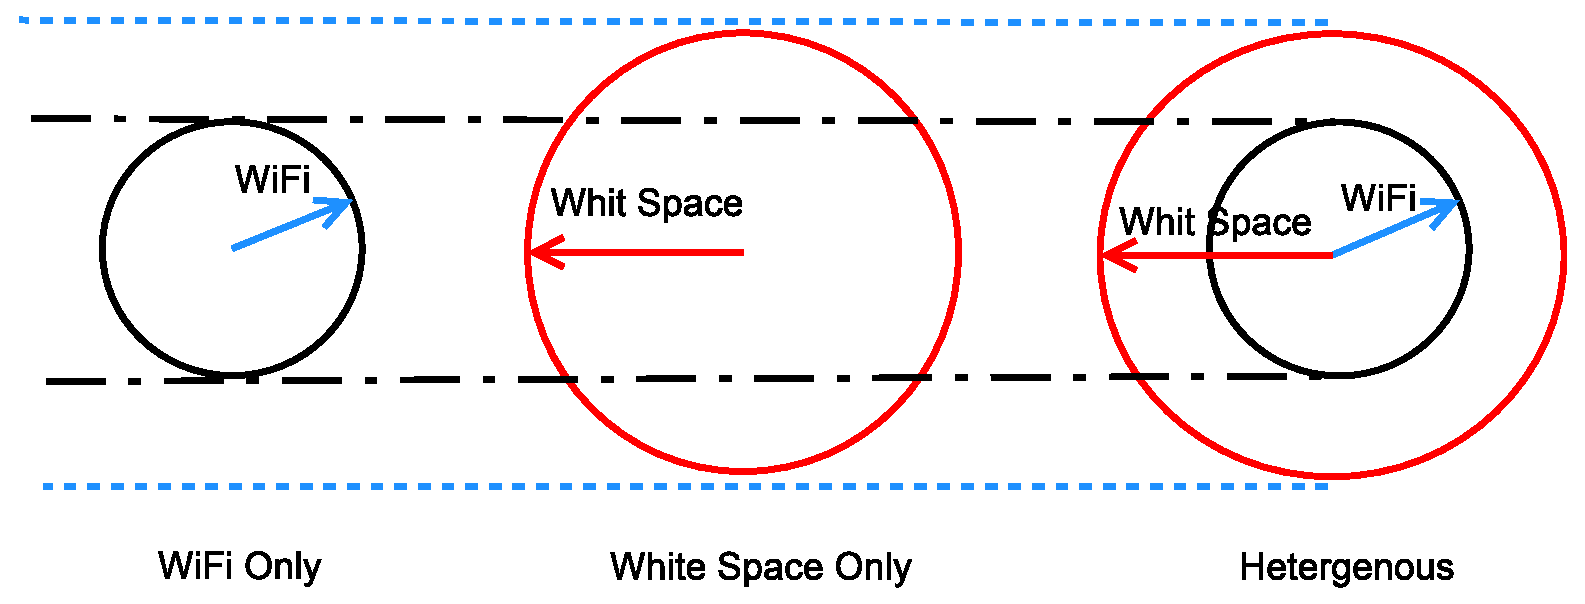
\includegraphics[width=84mm]{figures/lowtraffic}
\vspace{-0.1in}
\caption{Low Traffic Scenario}                                                                 
\label{fig:lowtraffic}
\vspace{-0.1in}
\end{figure}

\begin{figure}[h]
%\vspace{-0.0in}
\centering
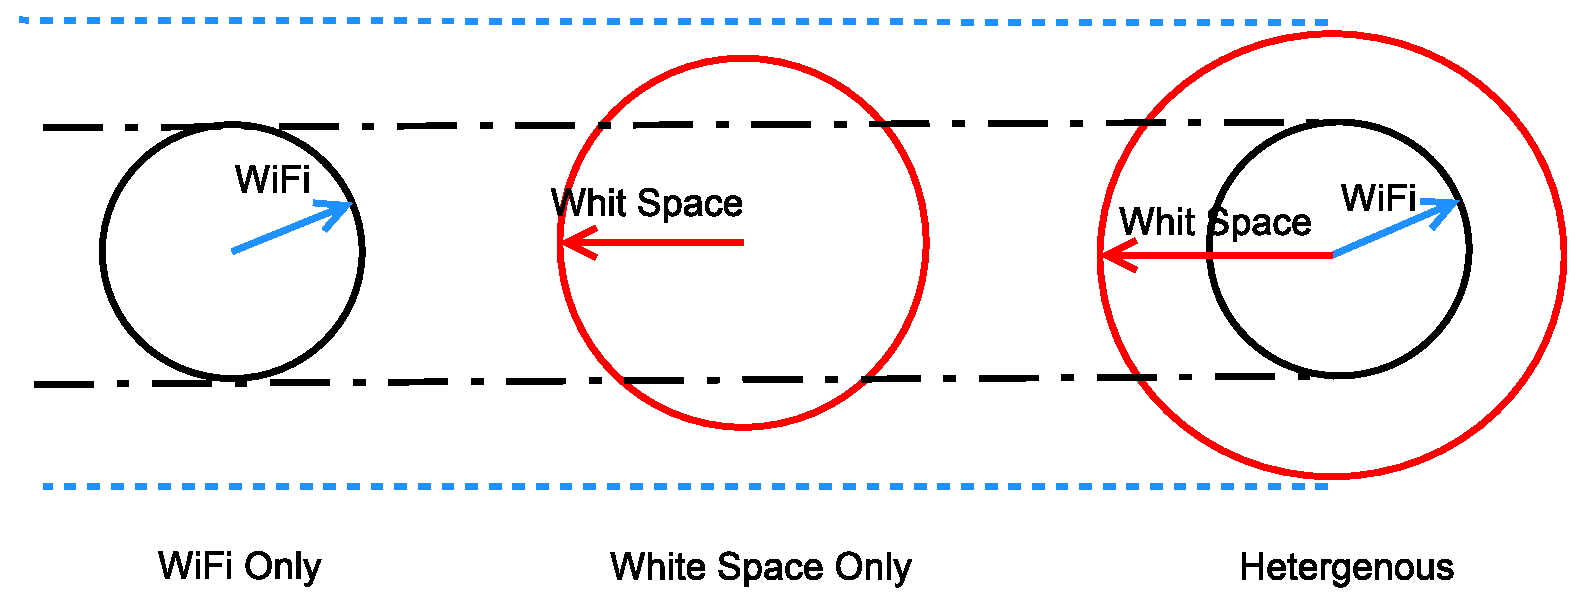
\includegraphics[width=84mm]{figures/mediumtraffic}
\vspace{-0.1in}
\caption{Medium Traffic Scenario}                                                                 
\label{fig:mediumtraffic}
\vspace{-0.1in}
\end{figure}


\begin{figure}[h]
%\vspace{-0.0in}
\centering
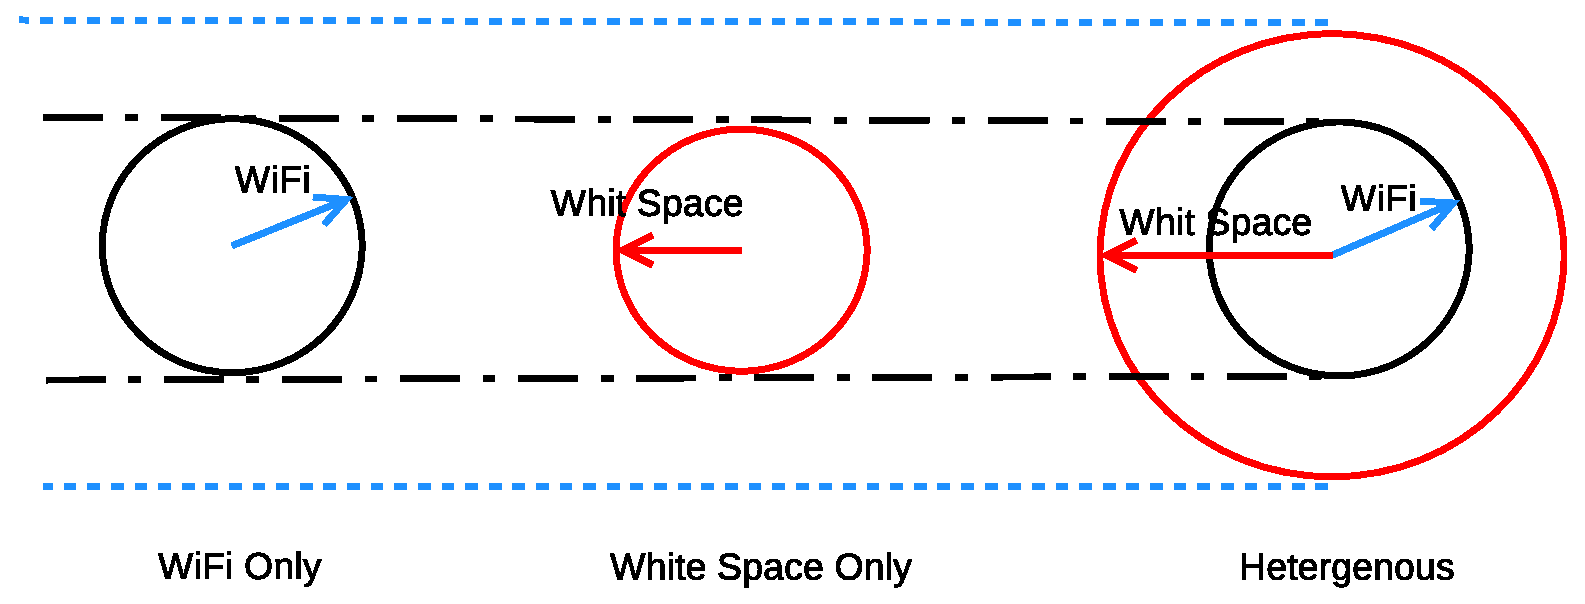
\includegraphics[width=84mm]{figures/hightraffic}
\vspace{-0.1in}
\caption{High Traffic Scenario}                                                                 
\label{fig:hightraffic}
\vspace{-0.1in}
\end{figure}

% Relaxed linear program
Given a target area $G$ with the traffic demand distribution $\gamma$, the service area 
of all kinds access points $S_t$, the coverage rate $p$, thus the capacity of access point $C_t$ could 
be calaculated based on the number of radios, Friis model~\ref{eq:friis} and restriction~\ref{eq:servicearea}
or from in-field measurement~\cite{cuileveraging}. When the target area is served, the reward of the area 
could be knows as a constant number $R$. However, the reward does not influence the optimal deployment since 
the total reward is a constant. Furthermore, the minimum number of access points could be found through 
a relaxed linear program as fllowing. 

\noindent
{\bf Sets:}
\begin{tabular}{ll}
$B$ & Set of Bands \\
$T$ & Type of Access Point\\
\end{tabular}

\noindent
{\bf Parameters:}\\
\\
%\vspace{0.1in}
%\begin{tabular}{lll}
\begin{tabular}{llp{3.4cm}}
$G$ &  & Target Area\\
$\gamma$ & & Traffic Demand Distribution\\
$p$ & & Coverage Rate\\
$S_t$ & $t \in T$ & Coverage Area of Type t AP\\
$O_{b,t}$ & $b \in B, t \in T\ binary$ & Channel Occupied by Type t AP\\
$N_b$ & $b \in B\ $ & Available channel of a band in Target Area\\
$C_t$ & $t \in T$ & Channel capacity of Type t AP\\
\end{tabular}


\noindent
%\vspace{2pt}
{\bf Variables:}\\
\\
%\vspace{1pt}
\begin{tabular}{llr}
$a_t\ge0$ & $t \in T$ & Number of Type t AP\\ 
\end{tabular}

\noindent
{\bf Objective:}
\begin{align}
& Min \sum_t a_t
\end{align}

\noindent
%{\bf Constraints:}
{\bf Coverage Constraint:}
\begin{align}
\label{opt:coverage}
\sum_t a_t\cdot S_t \ge G*p
\end{align}
\noindent
{\bf Capacity Constraint:} 
\begin{align}
\label{opt:capacity}
\sum_t a_t\cdot C_t \ge G\cdot \gamma
\end{align}
\noindent
{\bf Resource Constraint:} 
\begin{align}
\label{opt:resource}
\sum_t a_t\cdot O_{b,t} \le N_b
\end{align}

{\bf Spatial Constraint:} 
\begin{align}
\label{opt:resource}
a_t < \frac{G}{S_t}\cdot\frac{2}{3}\cdot N_b
\end{align}


The linear program relax the coverage constraint without telling a key parameter
{\it where should we put the access point?}. Moreover, the linear program may provide 
multiple results since different type of access points could have the same service area, 
(e.g. in low traffic demand case) The result of the linear program is the lower bound of 
access points. 

In order to find a pratical access points deployment in multiband scenario, we represent 
a greedy local search algorithm in~\ref{alg:gls}. The service area of access points varies 
from population distribution. Assume the cost of building an access point is the same as $C_a$. 
When an access point is built, the more service area is better. Thus hetegenous access point
could always have better performance. However, since there are a limit number of spectrum resource,
we have to balance the usability of hetegenous access point who reduce the cost of building access 
points, and single radio access point who may cover more areas.

In linear program, the reward $R$ is a constant of the area $G$. But for a single hetergenous access
point deployment, we have to compare its reward and cost to seperately using the radios.
In a certain area, a hetegenous AP has radius $r_1$. If we sperately using the radios with
radius $r_2,r_3,\dots r_n$, the reward is uniformly distributee, the hetegenous reward is defined as:

\begin{equation}
\label{eq:unitprice}
H_r=(n-1) C_a - \frac{R}{G}\cdot\sum f_s(r_n)
\end{equation}

$f_s(r)$ is the area calculation function, e.g. $f_s = \frac{3\sqrt{3}}{2}r^2$ when a 
hexagon coverage model is applied. In the framework, the access point type with more reward 
is going to deployed first till the available resource is used up. When two types of access points
share the same unit price, considering the spacial reuse, access point with high frequency channels
will be chosen. The deployment starts from the edge of the given plane and we use protocol model
to find the available access point type. If the combination of unit 
grid could be covered by an access point, we put the unit grid in the coverage area, until the access
point can not access more grid. Then we switch to another available access point. The process is like
a Teris game, when a given access point is filled, it will be deleted.
% Algorithm for lower bound approaching
\begin{algorithm}
\caption{Multiband Hetegeneous AP Deployment}
\label{alg:gls}
\begin{algorithmic}[1]
\REQUIRE  ~~\\
$G$: Target Area \\
$R$: Reward of Target Area \\
$\gamma$: Traffic Demand Distribution\\
$p$: Coverage Rate\\
$S_t$: Coverage Area of Type t AP \\
$O_{b,t}$: Channel Occupied by t Type AP\\
$N_b$: Available channels of a Band in Target Area\\
$C_t$: Channel Capacity of Type t AP
\WHILE {$\sum A\cdot S_t < p$}
\STATE Rank available AP type according to their unit price $H_r$
\STATE Rank available AP type according to radio numbers
\IF {The reminder area $G_r$ is larger than all the available AP}
\STATE Choose the AP has the largest coverage area $S_t$
\ELSE 
\STATE Find the available AP type whose coverage area $S_t=min{S_t>G_r}$
\ENDIF
\STATE Deploy an AP at the left up edge of un-covered area
\STATE Fill the AP with one neighbor unit grid and move the AP in the center of the coverage area
\STATE Update Channel Resource $O_{b,t}, N_b$
\STATE Update Output Access Point $A$
\ENDWHILE
\ENSURE ~~\\
The number of Access Points and Deployment\\
\end{algorithmic}
\end{algorithm}
% Algorithm analysis and justify

Generally, we employ access point with larger coverage capacity fill in the area, then for the 
Through the algorithm, we could cover the target area by the most efficient access point type
step by step. The minmum number of access points and a pratical multiband wireless deployment.
